\chapter{VTP}
\section{Overviews}
VLAN trunking protocol (VTP) allows a network administrator to manage VLANs on a switch configured as a VTP server. The VTP server distributes and synchronizes VLAN information over trunk links to VTP-enabled switches throughout the switched network. The following provides a brief description of important components of VTP:

\begin{itemize}
\item \textbf{VTP domain} consists of all interconnected switches. All switches in a domain share VLAN configuration details. Switches resides in different domains do not exchange VTP messages. The boundary of a VTP domain is a router or a layer-3 switch.

\item \textbf{Revision number} is a 32-bit number that indicates the level of revision for a VTP advertisements. Each VTP device tracks the VTP configuration revision number that is assigned to it. Each time that you make a VLAN change in a VTP device, the configuration revision is incremented by one. Therefore, this number is used to determine whether the received information is more recent than the current version.

\item \textbf{Password:} Switches in the same domain are configured with the same password for security reason.

\item \textbf{VTP modes:} A switch can be configured as a VTP server, client, or transparent.

\item \textbf{VTP server} stores the VLAN information in NVRAM (\verb|vlan.dat|), then advertises it to other switches. VLAN configuration is allowed, and affects the entire VTP domain.

\item \textbf{VTP client} stores the VLAN information in RAM, therefore, a switch reset deletes all VLAN information. VLAN configuration is not allowed.

\item \textbf{VTP transparent} does not allow switches to participate in VTP except to forward VTP advertisements to VTP clients and VTP server. VLANs that are created, renamed, or deleted on transparent switches are local to that switch only.
\end{itemize}

Each switch in a VTP domain sends periodic VTP advertisements so that its neighbors can update VLAN configuration. VTP includes three types of advertisements:

\begin{itemize}
\item \textbf{Summary advertisements} -- These inform adjacent switches of VTP domain name and configuration revision number. By default, Cisco switches issue summary advertisements \emph{every five minutes}. 
\item \textbf{Advertisement request} -- These are in response to a summary advertisement message when the summary advertisement contains a higher configuration revision number than the current value.
\item \textbf{Subset advertisements} -- These contain VLAN information including any changes.
\end{itemize}

\section{Operations}

When the switch receives a summary advertisement packet, it compares the VTP domain name to its own VTP domain name. If the name is different, the switch simply ignores the packet. If the name is the same, the switch then compares the configuration revision number of the packet to its own. If the switch's revision number is lower, it means that its VLAN database is out-dated, and it sends an advertisement request to ask for updates (subset advertisement messages). If the switch's revision number is \emph{not lower} to that of the packet, then the packet is ignored. \\

The configuration revision number reports any VLAN changes. When you add, delete, or change a VLAN on the VTP server, the VTP server increments the configuration revision. Then, the VTP server issues summary advertisements to announce that there have been some changes occur. Next, subset advertisements that contain information about these changes are sent to all VTP clients. This process is shown in the figure \ref{VTP-operation}.\\

\begin{figure}[hbtp]
\centering
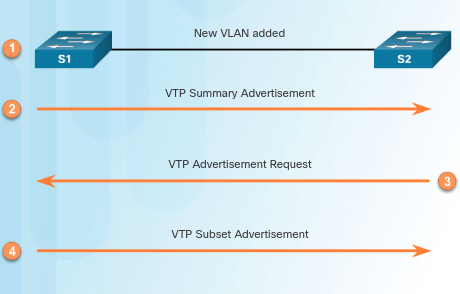
\includegraphics[width=0.6\textwidth]{pictures/VTP-operation.png}
\caption{VTP operation}
\label{VTP-operation}
\end{figure}

\section{VTP Caveats}

Suppose there is a new switch with a higher configuration revision number, and you want to install it into the existing switched network. Then, the existing VLAN configurations will be wiped out (see figure \ref{VTP-caveats}). Therefore, when a switch is added to a network, ensure that it has a default VTP configuration, or its revision number is reset to 0.\\

\begin{figure}[hbtp]
\centering
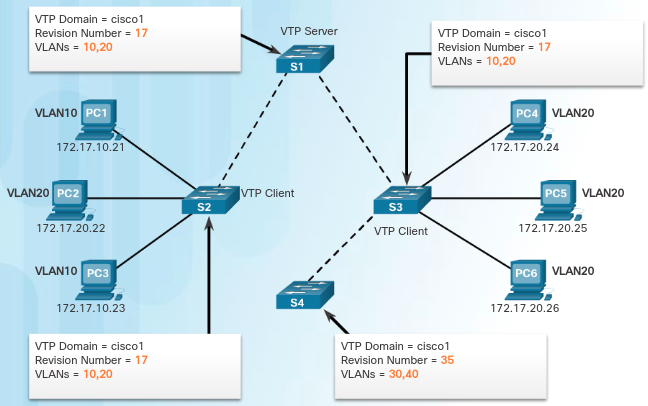
\includegraphics[width=0.8\textwidth]{pictures/VTP-caveats.png}
\caption{Incorrect VTP configuration revision number scenario}
\label{VTP-caveats}
\end{figure}

The VTP configuration revision number is stored in NVRAM and is not reset if you erase switch configuration and reload it. To reset VTP configuration revision number to zero you have two options:

\begin{itemize}
\item Change the switch's VTP domain to a nonexistent VTP domain and then change the domain back to the original name.
\item Change the switch's VTP mode to transparent and then back to previous VTP mode (Recommended).
\end{itemize}
